\documentclass[manuscript]{acmart}

\usepackage{tikz}
\usetikzlibrary{arrows.meta,positioning}

\setcopyright{none}
\settopmatter{printacmref=false}
\renewcommand\footnotetextcopyrightpermission[1]{}

\AtBeginDocument{%
  \providecommand\BibTeX{{Bib\TeX}}%
}

\title{AirDesk: Mid-Air Gestures for Situationally Impaired Desktop Interaction}

\author{Caden Calderon}
\affiliation{%
  \institution{Colorado State University}
  \city{Fort Collins}
  \state{Colorado}
  \country{USA}
}
\email{TODO}

\author{TODO Roommate Participant or Acknowledgment}
\affiliation{%
  \institution{Independent pilot participant}
  \city{TODO}
  \state{TODO}
  \country{USA}
}

\renewcommand{\shortauthors}{Calderon}

\begin{abstract}
AirDesk is a webcam-based prototype for controlling a Hyprland Linux desktop with mid-air hand gestures. The project is motivated by situationally impaired interaction: moments when keyboard and mouse input is unavailable, undesirable, dirty, painful, or physically costly. AirDesk does not try to replace traditional desktop input. Instead, it explores whether a small, clutch-based gesture vocabulary can work as a secondary control channel for coarse commands such as workspace switching, focus movement, and pause or cancel actions. This paper describes the AirDesk system, gesture vocabulary, safety model, logging and replay pipeline, and a small pilot evaluation with the project developer and one additional participant. Early prototype evidence suggests that naive rule-based recognition is not reliable enough for natural dynamic swipes. It also shows why fixed sliding-window recognition is a poor fit for continuous command streams: windows can cut gestures apart, merge adjacent gestures, or include background motion. DTW, motion-based spotting, and a newer TCN v2 recognizer are treated as competing pilot candidates until fresh continuous-session evidence shows which one is reliable enough to use. The paper contributes a focused system design and an evidence-bounded evaluation plan for mid-air desktop control under situational impairment.
\end{abstract}

\begin{CCSXML}
<ccs2012>
 <concept>
  <concept_id>10003120.10003121.10003122.10010854</concept_id>
  <concept_desc>Human-centered computing~Interaction techniques</concept_desc>
  <concept_significance>500</concept_significance>
 </concept>
 <concept>
  <concept_id>10003120.10003121.10003122.10003334</concept_id>
  <concept_desc>Human-centered computing~User interface design</concept_desc>
  <concept_significance>300</concept_significance>
 </concept>
 <concept>
  <concept_id>10003120.10003121.10003125.10011752</concept_id>
  <concept_desc>Human-centered computing~HCI design and evaluation methods</concept_desc>
  <concept_significance>300</concept_significance>
 </concept>
</ccs2012>
\end{CCSXML}

\ccsdesc[500]{Human-centered computing~Interaction techniques}
\ccsdesc[300]{Human-centered computing~User interface design}
\ccsdesc[300]{Human-centered computing~HCI design and evaluation methods}

\keywords{mid-air gestures, situational impairment, desktop interaction, hand tracking, Hyprland, 3D user interfaces, multimodal interaction}

\begin{document}
\maketitle

\section{Introduction}

Keyboard and mouse input are still excellent for most desktop work. They are precise, familiar, and fast. The problem is that people do not always use desktops under ideal conditions. A user may be cooking while following instructions on a monitor, painting or soldering with dirty hands, wearing gloves, standing away from a desk during a presentation, or avoiding repeated wrist movement during a long work session. In those moments, even simple operations such as switching workspaces, pausing media, moving window focus, or cancelling a command can become awkward.

AirDesk explores whether webcam-based mid-air hand gestures can help in these situations. The goal is not to replace keyboard and mouse input during normal desktop work. Instead, AirDesk focuses on coarse commands where availability matters more than precision: moving between workspaces, changing focus, pausing or cancelling the recognizer, and eventually controlling small profile-specific actions. A useful AirDesk command does not need to beat a keyboard shortcut when someone is already sitting at the keyboard. It needs to be available when touching the keyboard or mouse is inconvenient.

This paper presents AirDesk as a system paper with pilot evidence. The prototype is a Python-based webcam-to-desktop pipeline for Hyprland Linux. It includes camera capture, MediaPipe hand tracking, normalized hand-state events, command-mode gesture policy, dry-run action routing, guarded Hyprland dispatch, replayable JSONL logs, labeling tools, feature export, and offline recognizer evaluation. The evaluation is intentionally formative: the project developer and one roommate participant are used to identify which parts of the interaction are promising and which parts are not yet reliable enough for live desktop control.

This paper makes three contributions. First, it describes a safety-conscious interaction design for mid-air desktop commands based on explicit clutching, a small gesture vocabulary, dry-run defaults, and recovery gestures. Second, it documents a prototype pipeline that records, replays, labels, and evaluates hand-tracking sessions without repeatedly re-performing gestures. Third, it reports early prototype evidence showing how the recognizer evolved from simple rules, to DTW and motion baselines, toward a continuous TCN v2 spotting architecture.

\section{Related Work}

\subsection{Situational and Ability-Based Input}

Situationally induced impairments and disabilities describe contexts where environmental or temporary constraints make ordinary input harder to use \cite{sarsenbayeva2019siids}. Much SIID work is mobile-centered, but the idea also fits desktop computing. A keyboard and mouse may be physically present, yet still be a poor fit when a user's hands are dirty, gloved, occupied, painful, or far away from the desk. AirDesk uses this framing to motivate optional desktop gestures without treating them as universally better input.

Ability-based design provides the accessibility frame for this project. Rather than assuming one ideal input method, ability-based systems adapt to what users can do in a given context \cite{wobbrock2011ability}. AirDesk is best understood as an additional ability-aware input mode. It is accessibility-motivated, but this paper does not claim that AirDesk has been validated for any specific disability population. The current pilot can evaluate prototype feasibility and perceived usefulness under simulated constraints. Broader accessibility claims would require studies with the relevant users.

\subsection{Mid-Air Gesture Design}

Prior work on mid-air interaction shows both the appeal and difficulty of gesture input. Mid-air gestures can be expressive and easy to demonstrate, but their usability depends heavily on the application, task, evaluation method, feedback, training, prior experience, and participant factors \cite{koutsabasis2019empiricalmidair,catalano2025usablewithouttouch}. Gesture elicitation work also pushes against the idea of a universal mid-air vocabulary. Vogiatzidakis and Koutsabasis report that gesture identification depends on context of use \cite{vogiatzidakis2018gestureelicitation}, while Aigner et al. show that preferred gesture types vary by intended meaning and action \cite{aigner2012midairgestures}. Work on wall-display gestures makes the same point in another setting: the display and task shape the gesture set \cite{wittorf2016wallgestures}.

AirDesk applies these findings by choosing a small vocabulary for desktop commands instead of importing a broad gesture set from another domain. Workspace navigation maps naturally to directional swipes, focus movement can use short pointing-like gestures, and cancel or exit actions need a distinct recovery gesture. The design goal is not to find a universal vocabulary. It is to choose a vocabulary that is plausible, learnable, and measurable for AirDesk's desktop-command setting.

\subsection{Interaction Costs and Intent}

Mid-air input also has real costs. Hincapie-Ramos et al. show that upper-limb fatigue is a measurable design issue in mid-air interaction \cite{hincapie2014consumedendurance}. Error-prone in-air recognizers can affect user behavior and perceived control, especially when errors come from both human performance and system ambiguity \cite{arif2014errorprone}. These concerns matter for desktop control because a false activation can change the user's actual workspace.

Prior systems have handled unintended activation by separating activation gestures from command gestures. For example, mid-air smart-home control work uses registration gestures to decide which device should respond before accepting commands \cite{vogiatzidakis2020homedevices}. Public-display selection work also emphasizes clear phases and immediate feedback \cite{walter2014cuenesics}. AirDesk uses the same basic idea: an open-palm clutch enters listening mode, the recognizer accepts a short command gesture, and the system exits or cools down after the command. Continuous hand motion should not be treated as continuous command input.

Work comparing touch and mid-air interaction also supports AirDesk's secondary-channel framing. Jakobsen et al. found that touch can outperform mid-air for direct target acquisition, but users become more willing to choose mid-air as the movement cost of touch increases \cite{jakobsen2015touchmidair}. AirDesk follows that logic for desktop input. The important question is not whether a gesture beats a keyboard shortcut under ideal desk conditions. The question is whether a gesture becomes useful when ordinary input becomes costly.

\subsection{Recognition and Implementation Background}

AirDesk uses MediaPipe Hand Landmarker as its first hand-tracking backend \cite{zhang2020mediapipehands}. MediaPipe provides practical RGB hand landmarks, but it is not the contribution of this paper. The contribution is the desktop-control system built around tracking: safety policy, mode handling, replayable logs, labeling, and evaluation.

For gesture recognition, AirDesk separates static pose primitives, rule-based dynamic phrases, template or DTW matching, deterministic motion spotting, and learned temporal models. Template-based recognizers have a long history in HCI prototyping, including Wobbrock et al.'s work comparing simple recognizers with DTW and other baselines \cite{wobbrock2007dollar}. Temporal convolutional networks are useful for action segmentation and detection because they can model evidence over time rather than treating each frame in isolation \cite{lea2017tcn}. AirDesk uses this distinction to keep model claims honest: rules and DTW are practical baselines, while TCN v2 is an architecture for continuous gesture spotting that still needs fresh pilot evidence before it can drive live commands.

A key recognition challenge is the sliding-window problem. Many prototype recognizers classify a fixed window of recent frames. That works best when the gesture has already been neatly clipped, but live desktop control is not neatly clipped. A window may contain only the first half of a swipe, the end of one gesture plus the beginning of the next, or ordinary hand motion that happens to look gesture-like. Increasing the window size can capture more context, but also adds latency and makes repeated gestures blur together. Decreasing it improves responsiveness, but makes partial gestures more likely. AirDesk's TCN v2 direction is motivated by this trade-off: the model can still use a causal rolling window as context, but the window should not be treated as the gesture itself.

\section{Design Goals and Research Questions}

AirDesk is built around four design goals.

\textbf{G1: Support coarse desktop commands rather than precision input.} The first target actions are workspace movement, focus movement, pause/cancel, and profile-specific commands. These actions are useful enough to evaluate, but they do not require mouse-level precision or text entry.

\textbf{G2: Require explicit user intent before executing commands.} The system should not interpret every visible hand movement as a command. AirDesk uses a clutch/listen phase so that command gestures happen inside a short intentional window.

\textbf{G3: Make live desktop control safe to test.} Recognizer errors can affect the real desktop, so AirDesk defaults to dry-run routing, logs actions before execution, and limits guarded execution to allowlisted non-destructive Hyprland dispatchers.

\textbf{G4: Make recognition behavior replayable and measurable.} Gesture systems are easy to demo and hard to trust. AirDesk records hand-state streams, runtime events, labels, features, and evaluation outputs so recognizers can be tested against the same sessions. This is especially important for continuous gesture spotting, where window accuracy can look good even when event timing, repeated gestures, or background rejection fail.

These goals lead to the following research questions for the formative pilot:

\begin{enumerate}
  \item Can a small open-palm-clutched gesture vocabulary support common desktop command actions with acceptable false activation, latency, and perceived control?
  \item Which commands and recognizers are promising enough for future evaluation, and which fail under natural desktop motion?
  \item How does gesture control compare with keyboard/mouse input for coarse commands in a simulated situational impairment context?
\end{enumerate}

\section{System Overview}

AirDesk is implemented as a Python prototype with a modular pipeline. Hyprland is the initial desktop target because it exposes workspace and focus commands through dispatcher actions \cite{hyprlanddispatchers}.

\begin{figure}[h]
  \centering
  \resizebox{\linewidth}{!}{%
  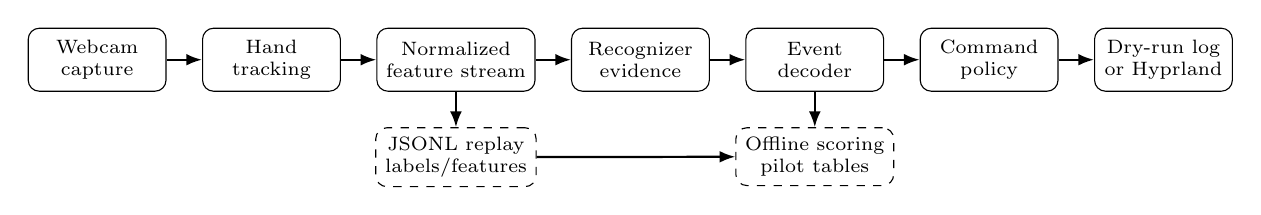
\begin{tikzpicture}[
    node distance=0.45cm,
    stage/.style={draw, rounded corners, align=center, minimum width=1.75cm, minimum height=0.8cm, font=\scriptsize},
    artifact/.style={draw, dashed, rounded corners, align=center, minimum width=1.9cm, minimum height=0.7cm, font=\scriptsize},
    arrow/.style={-{Latex[length=2mm]}, thick}
  ]
    \node[stage] (camera) {Webcam\\capture};
    \node[stage, right=of camera] (tracking) {Hand\\tracking};
    \node[stage, right=of tracking] (features) {Normalized\\feature stream};
    \node[stage, right=of features] (evidence) {Recognizer\\evidence};
    \node[stage, right=of evidence] (decoder) {Event\\decoder};
    \node[stage, right=of decoder] (policy) {Command\\policy};
    \node[stage, right=of policy] (action) {Dry-run log\\or Hyprland};

    \node[artifact, below=of features] (replay) {JSONL replay\\labels/features};
    \node[artifact, below=of decoder] (eval) {Offline scoring\\pilot tables};

    \draw[arrow] (camera) -- (tracking);
    \draw[arrow] (tracking) -- (features);
    \draw[arrow] (features) -- (evidence);
    \draw[arrow] (evidence) -- (decoder);
    \draw[arrow] (decoder) -- (policy);
    \draw[arrow] (policy) -- (action);
    \draw[arrow] (features) -- (replay);
    \draw[arrow] (replay) -- (eval);
    \draw[arrow] (decoder) -- (eval);
  \end{tikzpicture}}
  \caption{AirDesk's current architecture. The live path moves from webcam frames to guarded desktop actions, while the same feature and event streams feed replay, labeling, and offline evaluation.}
  \label{fig:pipeline}
\end{figure}

The current prototype includes OpenCV camera capture, MediaPipe hand tracking, replayable JSONL recordings, a replay backend, typed profile files, static gesture primitives, command-mode policy, dry-run action routing, guarded Hyprland dispatch, cursor-control experiments, label files, feature export, and offline gesture evaluation. Figure~\ref{fig:pipeline} shows the main architecture.

\subsection{Pipeline Components}

The capture layer reads webcam frames through OpenCV. The first tracking backend uses MediaPipe to infer hand landmarks from RGB frames. AirDesk converts those landmarks into normalized hand-state records with timing, hand presence, landmark positions, and derived pose features. This normalization step keeps the rest of the system from depending too tightly on MediaPipe. Future depth cameras or alternative hand trackers could emit the same hand-state shape.

The recognition layer converts hand states into candidate gesture events. Static primitives identify hand configurations such as open palm, fist, pointing, and pinch. Dynamic recognizers evaluate motion over short windows for actions such as left and right swipes. The policy layer then decides whether a gesture matters in the current mode. For example, a swipe outside command mode should be logged as background motion, not executed as a workspace command.

The action layer maps accepted commands to either dry-run logs or guarded Hyprland dispatches. Hyprland is a useful first target because workspace and focus actions are already exposed through dispatcher commands. That makes real desktop control testable without writing a custom window manager integration. AirDesk keeps this layer replaceable so other desktops or action targets can be added later.

\section{Interaction Design}

\subsection{Command Mode and Safety}

Safety is central because false activations can affect the real desktop. AirDesk defaults to dry-run execution, logs events, and requires explicit opt-in for real Hyprland actions. The command-mode profile uses an open-palm clutch to enter listening mode, then accepts a small set of commands before exiting or cooling down. In the current prototype, real execution is allowlisted and non-destructive.

The clutch is also an interaction design choice. It gives the user a visible boundary between ordinary motion and command motion, and it gives the recognizer a shorter window to inspect. This matters in a webcam setting, where normal desk motion such as reaching for a phone, adjusting posture, or moving near the keyboard can resemble parts of a command gesture.

\subsection{Gesture Vocabulary}

The current command vocabulary is intentionally small:

\begin{itemize}
  \item open palm hold: enter listening mode;
  \item fist: cancel or exit command mode;
  \item swipe left/right: workspace navigation candidate;
  \item point left/right: focus movement candidate;
  \item pinch: cursor-mode or confirmation primitive in separate modes.
\end{itemize}

This vocabulary emphasizes coarse command actions rather than text entry or continuous precision pointing.

\subsection{Feedback and Recovery}

AirDesk treats recovery actions as part of the core vocabulary rather than as an afterthought. A command system that can switch workspaces or change focus must give users a way to stop listening, cancel an uncertain command, and recover from accidental recognition. The current design includes pause/cancel behavior and cooldowns after accepted commands. The pilot will pay attention not only to whether intended commands fire, but also to whether participants feel they can keep the system under control.

\section{Implementation and Reproducibility}

\subsection{Runtime and Profiles}

The implementation is organized as a Python command-line prototype. Runtime commands can capture live webcam input, replay recorded sessions, route recognized events to dry-run output, or invoke guarded Hyprland dispatchers. Profiles define which gestures are active, how they map to actions, and whether the system is operating in dry-run or execution mode.

The default safety posture is dry-run-first. This lets AirDesk show what would have happened without actually changing the desktop. For live execution, the dispatcher layer is intentionally narrow: only explicit, non-destructive actions such as workspace movement and focus movement are candidates for guarded execution.

\subsection{Logging, Replay, and Labeling}

AirDesk records normalized tracking frames and runtime events as JSONL. Replay support allows recognizer changes to be evaluated without repeatedly performing gestures. The labeling workflow creates per-recording JSON label files with event and phase labels, then exports deterministic landmark-derived feature CSVs for evaluation and future model training.

This replay workflow makes the system easier to evaluate honestly. A recognizer can be changed, tuned, or replaced, then tested against the same recorded sessions. The final submission package will include the LaTeX source, literature PDFs, README links, and enough project documentation to locate the code, recordings, labels, features, and evaluation summaries used in the report.

\subsection{Recognizer Evolution}

AirDesk's recognizer changed as the project moved from isolated gestures toward continuous desktop use. This shift was partly motivated by prior project experience with an LSTM-based smart-home gesture recognizer. That recognizer used a traditional sliding window over recent frames. It could work when the window happened to contain a full gesture, but it was fragile when the timing was not perfect. Sometimes the window captured only part of the gesture. Sometimes it included the reset motion after the gesture. Sometimes it caught the end of one gesture and the start of the next. It was also slower than desired for interactive control.

That experience shaped AirDesk's model search. The goal was not simply to find a higher-accuracy classifier, but to find a recognizer that could handle fast commands, repeated gestures, and short chains without requiring a long pause between actions. DTW and TCNs became the two practical directions. DTW is useful because it aligns variable-length motion traces and can work with a small number of personal examples. A causal TCN is useful because it can process a stream with explicit, bounded latency rather than waiting for a recurrent model to summarize the sequence.

The first AirDesk dynamic recognizer was rule-based: it looked for simple motion patterns over a recent time window and emitted a swipe when the motion crossed a threshold. This was easy to inspect, but it failed under natural motion. Normal desk activity could look enough like a command to trigger false activations, while some real swipes were missed because tracking dropped or the hand did not move in the exact expected way.

The next step was a DTW-style template baseline. DTW is practical for a small personal vocabulary because it compares a new motion trace against examples instead of relying only on hand-written thresholds. However, DTW still depends on good segmentation. The system has to decide when a gesture starts and ends before comparing it to a template. In continuous use, that boundary problem is often the hard part.

The current TCN v2 direction is a response to the same boundary problem. The first learned AirDesk model still treated rolling windows too much like gesture clips: each window received one label, and the model tried to classify the window. That is a weak match for live desktop gestures. A real hand stream contains partial gestures, pauses, resets, fast repeated commands, tracking loss, and ordinary background motion. TCN v2 instead treats a rolling window as compute context. The model produces frame-level evidence such as intentional motion, left/right stroke evidence, and start/end boundaries. An event decoder then turns that evidence into one command event. The key design change is that the window provides context, but the emitted gesture is defined by evidence and boundaries rather than by the arbitrary start and end of a fixed buffer.

This does not mean TCN v2 is assumed to be the final recognizer. The final pilot should use whichever recognizer is most reliable after fresh continuous validation. If TCN v2 produces clean event-level behavior, it can become the pilot recognizer. If it remains underconfident or false-activation prone, a gated DTW or deterministic motion baseline is a better choice for the pilot, and TCN v2 should be reported as an architectural improvement and future-work path.

\subsection{Recognizer Baselines}

AirDesk currently uses four levels of recognition evidence. Static pose recognizers provide simple primitives such as open palm, fist, point, and pinch. Rule-based dynamic recognizers inspect recent hand motion to identify candidate swipes. A DTW-style template baseline compares observed motion against personalized examples. A TCN v2 sequence-evidence model is being prepared for continuous gesture spotting. The final evaluation should compare recognizers using event-level behavior: matches, misses, false activations, repeated fires, latency, and sequence order. Clip accuracy alone is not enough for a desktop command system because it does not show whether commands can be chained, repeated, or rejected during normal background motion.

\section{Pilot Method}

\subsection{Participants}

The pilot will include the project developer and one roommate participant. This is a small formative pilot, not a generalizable user study. The participant count reflects the course timeline and solo-project constraints.

\subsection{Apparatus}

The pilot will run on the developer's Linux desktop using a commodity webcam and the AirDesk prototype. The current camera baseline is approximately 640 by 480 pixels at 30 FPS. Hyprland is the live desktop target, but dry-run logs will be used before any guarded live execution. The final paper will report the exact machine, webcam, lighting conditions, and AirDesk commit used for the pilot.

\subsection{Conditions and Tasks}

The intended conditions are:

\begin{itemize}
  \item keyboard/mouse baseline at the desk;
  \item AirDesk live dry-run;
  \item optional AirDesk guarded execution if dry-run behavior is stable;
  \item optional simulated situational impairment, such as standing away from the keyboard or wearing gloves.
\end{itemize}

Candidate tasks include switching workspace left, switching workspace right, moving focus left, moving focus right, cancelling command mode, and pausing or resuming the runtime. The final task set should stay small so the pilot evaluates command reliability rather than participant endurance. Text entry and small-target cursor manipulation are outside the main evaluation.

\subsection{Procedure}

Each participant will complete a short practice phase, a keyboard/mouse baseline, an AirDesk dry-run condition, and optionally a guarded-execution or simulated-impairment condition if dry-run behavior is stable. Participants will be told that the system is a prototype and can be stopped at any time. The session will stop if false activations repeatedly occur during normal motion, if the participant reports fatigue or discomfort, or if live execution controls the wrong target more than once.

\subsection{Measures}

Objective measures include task success, completion time, false activations, missed intended gestures, repeated fires, gesture-to-action latency, fallback keyboard or mouse use, and tracking loss. Subjective measures include perceived control, fatigue or discomfort, frustration, perceived usefulness, preference versus keyboard/mouse baseline, and short interview notes. The final analysis will report these values descriptively rather than using inferential statistics, because the pilot sample is too small for population-level claims.

\section{Prototype Evidence and Findings}

The current evidence comes from recorded local gesture sessions and replay evaluation. A Sprint 4 batch contains 24 recordings: eight left-swipe takes, eight right-swipe takes, and eight normal desk-motion negative takes. Labels, features, DTW models, TCN v2 manifests, and evaluation summaries were generated from those recordings. These data are not a substitute for the planned pilot, but they are useful for deciding which recognizer is credible enough to test.

\begin{table}[h]
  \caption{Current offline recognizer evidence from the Sprint 4 swipe batch. Same-batch DTW is optimistic because calibration and evaluation used the same small distribution. The gated holdout result was tuned after inspecting the split. The first TCN v2 model validates the training/evaluation surface, but does not yet provide usable event-level recognition.}
  \label{tab:offline-evidence}
  \centering
  \begin{tabular}{llll}
    \hline
    Recognizer & Positive matches & False activations & Mean latency \\
    \hline
    Rule swipe & 0/16 & high & n/a \\
    Same-batch DTW & 16/16 & 2 & 0.44s \\
    Initial holdout DTW & 2/4 & 0 & 0.40s \\
    Gated holdout DTW & 4/4 & 0 & 0.36s \\
    TCN v2 quick smoke & 1/16 & 2 & n/a \\
    \hline
  \end{tabular}
\end{table}

Rule-based dynamic swipe recognition performed poorly on this batch. It matched zero of sixteen intended positive swipe events and produced many false activations, especially from crude static-pose recognizers firing during natural motion.

A personalized DTW baseline performed better on the same batch, matching all sixteen intended swipes with two false activations and approximately 0.44 seconds mean latency. However, this same-batch result is optimistic because calibration and evaluation used the same small data distribution.

A deterministic holdout evaluation trained on takes 001--006 and tested on takes 007--008. The first holdout matched both right swipes but missed both left swipes, with no false activations on held-out negatives. A later horizontal-displacement-gated variant matched all four held-out swipes with no held-out false activations, but it was tuned after inspecting that split. The gated result is promising but should be validated on a fresh continuous chained recording before being used as live-control evidence.

The first TCN v2 smoke test shows the opposite kind of result. The data/model/evaluation surface works, and the model can be trained over frame-level evidence heads. However, the initial old-data model was underconfident at the event level. A permissive replay pass matched only one of sixteen intended swipes and produced two false activations. This result does not mean the TCN v2 direction is wrong. It means the architecture needs fresh continuous training data and event-level decoding before it can be compared fairly with DTW.

The pilot results will extend this evidence with live-session task outcomes and short interview notes. The main values to report are task success, false activations, missed gestures, repeated fires, completion time, perceived control, fatigue, and perceived usefulness. The qualitative summary will focus on which commands felt natural, which commands felt unreliable, and when participants would actually prefer AirDesk over keyboard or mouse input.

\section{Discussion}

AirDesk's current results support the project framing: the most valuable contribution so far is not a final gesture recognizer, but an instrumented system for making desktop gesture control measurable. The rule recognizer failure is useful because it shows that clean synthetic gestures are not enough. Natural desktop motion creates false activations, and dynamic command gestures require explicit intent gates, background rejection, and replay-based evaluation.

The DTW results suggest that personalized gesture templates may be viable for a small vocabulary, especially when combined with motion-direction gates. The TCN v2 work suggests a different lesson: the learned-model problem is not simply ``classify this window.'' The model and decoder have to spot gesture events inside a continuous stream. This matters because a desktop command system should allow repeated or chained gestures without forcing the user to pause until a fixed window resets. That is why the current paper should compare recognizers at the event level, not by window accuracy. The final pilot should use the most reliable recognizer available at that point, even if that is DTW rather than TCN v2.

The design also suggests a useful boundary for future development. Command mode is a better first paper target than cursor mode because workspace and focus actions are discrete, recoverable, and easy to log. Cursor takeover, click, drag, and text entry are more demanding because small errors are more disruptive and fatigue accumulates quickly. AirDesk can still grow into those modes, but the first evaluation should focus on commands that match the strengths of mid-air input.

Finally, the small pilot should be interpreted as a formative design check. If the roommate participant finds the clutch confusing, the gesture vocabulary tiring, or dry-run feedback hard to understand, those are valuable results. The goal is not to prove that AirDesk is finished. The goal is to identify the smallest credible desktop gesture loop that works well enough to justify broader evaluation.

\section{Limitations}

This project has several limitations. The pilot participant count is small, and one participant is the developer. The current hardware baseline is a commodity webcam at approximately 30 FPS, which may limit tracking quality under poor lighting, occlusion, or fast movement. The evaluation so far is developer-centered and may overfit to one user's gesture style. Dynamic gesture recognition is not yet validated for real-time live control in a fresh continuous session. Cursor mode exists as a guarded prototype but is not part of the main paper evaluation. Accessibility benefits are design motivations, not validated claims.

The recognizer evidence also has limits. Same-batch DTW results are optimistic, and the gated holdout result was tuned after observing the first holdout behavior. The current TCN v2 result is also preliminary: it validates the pipeline shape more than the recognition quality. These results are useful engineering signals, but the paper should not present them as final model performance. The final pilot should add fresh continuous motion and normal background activity before making any stronger reliability claims.

\section{Future Work}

Future work includes a larger participant study, improved continuous-session labeling, a stronger continuous-spotting recognizer, richer overlay feedback, safer real cursor click and drag injection, depth or Kinect context, and profile-specific gesture vocabularies for media, presentation, and accessibility use cases. A larger study should include participants who actually experience the target constraints rather than only simulating them. For example, future work could separately study gloves, distance-from-keyboard use, wrist-pain scenarios, and presentation contexts.

The system could also support user-specific calibration. The early DTW results suggest that personalized templates may work for a small vocabulary, but future versions should make calibration explicit, measure how many examples are needed, and determine whether templates transfer across days, lighting conditions, and camera positions. For TCN v2, the next step is not simply more epochs. It is better continuous data, reviewed labels, event-boundary evidence, and decoder thresholds that are evaluated on full streams. The long-term target is a recognizer that can handle partial gestures, adjacent gestures, and repeated commands without treating a fixed frame window as the unit of meaning.

\section{Conclusion}

AirDesk explores mid-air gestures as a secondary desktop command layer for situationally impaired interaction. The current prototype provides a pluggable architecture, explicit command mode, dry-run-first execution, replayable logs, labeling, feature extraction, and early recognition baselines. The system is strongest when framed as an optional command channel for moments when keyboard and mouse input is inconvenient, not as a replacement for ordinary desktop input. The main lesson so far is that credible desktop gesture systems need explicit intent, safety boundaries, and continuous-stream evaluation rather than isolated gesture demos. The planned pilot will use that framing to determine which recognizer and interaction loop are ready for broader evaluation and which should remain future work.

\bibliographystyle{ACM-Reference-Format}
\bibliography{references}

\end{document}
